% ch03 Born–Oppenheimer approximation (书页 16–23 / 分册p1–p8)
% 第3章 Born–Oppenheimer approximation
\chapter{玻恩–奥本海默近似}

在本章中，我们建立基本框架，用以考察电子–电子（e-e）、电子–离子（e-i）以及离子–离子（i-i）相互作用如何影响固体的性质。我们首先证明，电子与离子的自由度可以解耦。之所以能够这样分离，是因为在固体中离子和电子的速度相差极为悬殊：粗略地说，电子速度约为离子速度的1000倍。其结果是，在电子看来，离子提供了它们于其中运动的静态背景。这一物理图像正是玻恩–奥本海默近似（Born–Oppenheimer approximation）[BO1927]的核心。

\section{基本哈密顿量}

在开头先考虑总哈密顿量（Hamiltonian）是有益的，这有助于理解如何把电子运动与离子运动分离开来。我们用$\mathbf R_i$与$\mathbf P_i$分别标记第$i$个离子的位置与动量，用$\mathbf r_j$与$\mathbf p_j$标记第$j$个电子的位置与动量。我们假设所有离子的质量均为$M$，核电荷为$Ze$。总哈密顿量为

\begin{equation*}
\begin{aligned}
H = {} & \sum_i \frac{\mathbf P_i^2}{2M} + \sum_j \frac{\mathbf p_j^2}{2m} + \frac{(Ze)^2}{2}\sum_{i,i'} \frac{1}{|\mathbf R_i - \mathbf R_{i'}|} \\
& + \frac{e^2}{2}\sum_{j,j'} \frac{1}{|\mathbf r_j - \mathbf r_{j'}|} - Ze^2\sum_{i,j} \frac{1}{|\mathbf r_j - \mathbf R_i|}.
\end{aligned}
\tag{3.1}
\end{equation*}

这个哈密顿量不包含外电场或外磁场，也不包含各组分之间的磁相互作用。最后三项分别是i-i、e-e与e-i相互作用。为了在这一哈密顿量的基础上继续推进，我们按被束缚的程度把电子分成两组——芯电子（core electrons）与价电子或传导电子（valence or conduction electrons）。这一分离很有用，因为芯电子随原子核一起运动，而传导电子或价电子则在整个固体中输运。考虑到这一分离，我们得到如下分区哈密顿量（partitioned Hamiltonian）：

\begin{equation*}
\begin{aligned}
H = {} & \sum_i \frac{\mathbf P_i^2}{2M} + \sum_{j=\mathrm{cond.\,elec.}} \frac{\mathbf p_j^2}{2m} + \sum_{i,i'} V_{i,i'}(|\mathbf R_i - \mathbf R_{i'}|) \\
& + \frac{e^2}{2}\sum_{j,j'=\mathrm{cond.\,elec.}} \frac{1}{|\mathbf r_j - \mathbf r_{j'}|} + \sum_{i,j} V_{\mathrm{ei}}(|\mathbf r_j - \mathbf R_i|) + E_{\mathrm{core}}
\end{aligned}
\tag{3.2}
\end{equation*}

\begin{figure}[H]\centering
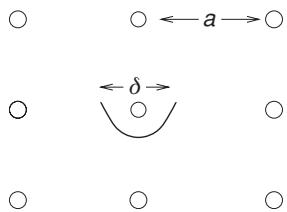
\includegraphics[width=0.45\textwidth]{figs/ch03/fig_3.1.jpg}
\caption*{图 3.1\quad 间距为$a$的离子晶格。每个离子在简谐势阱中振荡，其偏离自身原位的幅度相对于离子间距很小。偏离量大致为$\delta\sim(m/M)^{1/4}a\sim10^{-4}a$，其中$m$为电子质量，$M$为离子质量。正因如此，相对于电子自由度，离子基本上可以被当作固定不动。离子构成电子运动的一个固定的、几乎刚性的背景，这正是玻恩–奥本海默近似的精髓。}\label{fig:auto:3.1}
\end{figure}

在式 (3.2) 中，$V_{i,i'}$与$V_{\mathrm{ei}}$分别表示离子之间以及价电子与离子之间的有效势。芯电子的能量为$E_{\mathrm{core}}$。以Na为例，总的$Z$为11，轨道填充为$1s^2\,2s^2\,2p^6\,3s$，只有一个未配对的价电子。在这一表示中，离子的有效电荷为$Z=1$。

\section{绝热近似}

为简化式 (3.2)，我们把核的运动与电子的运动分离开来；由于离子比电子质量大得多，这一分离是合理的。典型值为$m/M\sim 1/2000$到$1/500\,000$。表征这一展开的小参量是$(m/M)^{1/4}$。下面我们将证明，离子速度通过比值$(m/M)^{3/4}$与费米速度（Fermi velocity）相联系。因此，相对于电子，离子可以基本上当作静止的。这使我们能够先假定离子固定在其平衡位置来求解电子运动，而离子运动的效应可以当作微扰（perturbation）来处理；也就是说，电子绝热地（adiabatically）调整以跟随离子运动。从离子的角度看，电子的快速运动产生一个它们所能感受到的总体平均电子势。这一分离正是玻恩–奥本海默近似的精髓。

为理解离子与电子的速度和能量的相对量级，我们为了论证起见假设每个离子各自在形如$V_{\mathrm{osc}}=M\omega^2R^2/2$的简谐势阱中运动（见图 3.1），其中$R$度量离子偏离其原位（即平衡位置）的距离。考虑把一个离子移动一个晶格间距$a$。这样做的能量代价$\sim M\omega^2a^2/2$，本质上就是使电子波函数发生畸变所需的能量，因而该能量为$\hbar^2/2ma^2$的量级，而这又与电子动能$p_{\mathrm F}^2/2m$同量级。于是$M\omega^2a^2/2\sim p_{\mathrm F}^2/2m$。对$\omega$求解，我们得到

\begin{equation*}
\omega \sim (m/M)^{1/2}\frac{\hbar}{ma^2},
\tag{3.3}
\end{equation*}

然而，对简谐势阱中的离子，$P^2/2M=\hbar\omega/2$，等价地说，离子速度的平方为$\hbar\omega/M$。把这一结果与前面关于$\omega$的结果结合起来，我们得到

\begin{equation*}
v_{\mathrm{ion}} \sim (m/M)^{3/4}v_{\mathrm F} \sim (10^{-2}\ \mathrm{to}\ 10^{-3})v_{\mathrm F}.
\tag{3.4}
\end{equation*}

我们来估计离子偏离其平衡位置有多远。对于位移 $\delta$，有 $M\omega^{2}\delta^{2}/2\sim\hbar\omega/2$。代入 $\omega\sim(m/M)^{1/2}\hbar/ma^{2}$，我们求得离子位移

\begin{equation*}
\delta \sim a(m/M)^{1/4} \sim 10^{-4}a,
\tag{3.5}
\end{equation*}

如图 3.1 所示，这个位移可以忽略不计。对电子而言，离子是静止的。我们可以按小量$\delta/a$即$(m/M)^{1/4}$展开微扰级数，来计算电子自由度所起的作用。还要注意，由于$P^2/2M\sim\hbar\omega/2\sim\epsilon_{\mathrm F}(m/M)^{1/2}\ll\epsilon_{\mathrm F}$，离子的动能相对较小。

玻恩–奥本海默近似的形式化推导从如下假设出发：全波函数是多电子位置$\mathbf r\equiv\{\mathbf r_j\}$与离子位置$\mathbf R\equiv\{\mathbf R_i\}$的函数，并且可以展开为

\begin{equation*}
\Psi(\mathbf r,\mathbf R) = \sum_n \Phi_n(\mathbf R)\Psi_{\mathrm e,n}(\mathbf r,\mathbf R),
\tag{3.6}
\end{equation*}

其中$\Psi_{\mathrm e,n}(\mathbf r,\mathbf R)$（以$n$标记）是离子位置$\mathbf R$固定时电子–离子问题的解。离子波函数$\Phi_n(\mathbf R)$一方面描述离子处于位置$\mathbf R$的振幅，另一方面又可以看作电子波函数的展开系数。$\Psi_{\mathrm e,n}$构成完备的正交归一集。于是，

\begin{equation*}
\int \mathrm d\mathbf r\, \Psi_{\mathrm e,n}^{*}(\mathbf r,\mathbf R)\Psi_{\mathrm e,m}(\mathbf r,\mathbf R) = \langle en|em\rangle = \delta_{nm}.
\tag{3.7}
\end{equation*}

再结合核波函数的正交性条件

\begin{equation*}
\int \mathrm d\mathbf R\, \Phi_n^{*}(\mathbf R)\Phi_m(\mathbf R) = \delta_{nm},
\tag{3.8}
\end{equation*}

完整的电子–离子波函数便是归一的：

\begin{equation*}
\langle \Psi(\mathbf r,\mathbf R)\,|\,\Psi(\mathbf r,\mathbf R)\rangle = 1.
\end{equation*}

我们由$\Phi_n$与$\Psi_{\mathrm e,n}$所服从的运动方程确定各个展开系数。为此，我们把式 (3.2) 改写为

\begin{equation*}
H = T_{\mathrm i} + T_{\mathrm e} + V_{\mathrm{ii}} + V_{\mathrm{ee}} + V_{\mathrm{ei}} + E_{\mathrm{core}},
\tag{3.9}
\end{equation*}

其中式 (3.9) 中的各项与式 (3.2) 中的各项一一对应。式 (3.9) 的本征值方程为

\begin{equation*}
(T_{\mathrm i} + T_{\mathrm e} + V_{\mathrm{ii}} + V_{\mathrm{ee}} + V_{\mathrm{ei}} + E_{\mathrm{core}})\Psi = E\Psi
\tag{3.10}
\end{equation*}

\begin{equation*}
(T_{\mathrm i} + V_{\mathrm{ii}} + E_{\mathrm{core}})\Psi + \sum_n \Phi_n(T_{\mathrm e} + V_{\mathrm{ee}} + V_{\mathrm{ei}})\Psi_{\mathrm e,n}(\mathbf r,\mathbf R) = E\Psi.
\tag{3.11}
\end{equation*}

我们注意到$T_{\mathrm e}+V_{\mathrm{ee}}+V_{\mathrm{ei}}$只作用于乘积波函数的电子部分，以此简化上式。令$E_{\mathrm e,n}(\mathbf R)$为核坐标固定时电子系统的能量。这样一来，核的本征值方程

\begin{equation*}
\sum_n \left(T_{\mathrm i} + V_{\mathrm{ii}} + E_{\mathrm{core}} + E_{\mathrm e,n} - E\right)\Phi_n\Psi_{\mathrm e,n} = 0,
\tag{3.12}
\end{equation*}

与电子的本征值方程

\begin{equation*}
(T_{\mathrm e} + V_{\mathrm{ee}} + V_{\mathrm{ei}})\Psi_{\mathrm e,n}(\mathbf r,\mathbf R) = E_{\mathrm e,n}(\mathbf R)\Psi_{\mathrm e,n},
\tag{3.13}
\end{equation*}

便可以分离开来。

我们用$\Psi_{em}^{*}=\langle em|\mathbf r,\mathbf R\rangle$乘以核的本征值方程并积分：

\begin{align*}
&\sum_n \int \mathrm d\mathbf r\, \Psi_{\mathrm e,m}^{*}(\mathbf r,\mathbf R)T_{\mathrm i}\Phi_n(\mathbf R)\Psi_{\mathrm e,n}(\mathbf r,\mathbf R) \\
&\qquad + \left(V_{\mathrm{ii}} + E_{\mathrm{core}} + E_{\mathrm e,m}(\mathbf R) - E\right)\Phi_m(\mathbf R) = 0.
\tag{3.14}
\end{align*}

由于矩阵元$\langle en|V_{\mathrm{ii}}(\mathbf R)|em\rangle$只涉及纯代数算符，它只有对角元。然而动能项具有非对角元；具体写出为

\begin{align*}
\sum_i \left\langle em\left|\frac{\mathbf P_i^2}{2M}\Phi_n(\mathbf R_i)\right|en\right\rangle &= -\frac{\hbar^2}{2M}\sum_i \int \mathrm d\mathbf r\, \Psi_{\mathrm e,m}^{*}(\mathbf r,\mathbf R)\Big[ \\
&\quad \big(\nabla_{\mathbf R_i}^2\Phi_n(\mathbf R)\big) + 2\big(\nabla_{\mathbf R_i}\Phi_n(\mathbf R)\big)\cdot\nabla_{\mathbf R_i} \\
&\quad + \Phi_n(\mathbf R)\nabla_{\mathbf R_i}^2\Big]\Psi_{\mathrm e,n}(\mathbf r,\mathbf R).
\tag{3.15}
\end{align*}

由于$\nabla_{\mathbf R}^2$在积分的第一项中只作用于$\Phi_n(\mathbf R)$，所得矩阵元是纯对角的。目前我们略去动能矩阵元中的后两项，得到

\begin{equation*}
\sum_n \left(T_{\mathrm i} + V_{\mathrm{ii}} + E_{\mathrm{core}} + E_{\mathrm e,n}(\mathbf R)\right)\Phi_n(\mathbf R) = \sum_n E_n\Phi_n(\mathbf R),
\tag{3.16}
\end{equation*}

或者等价地，

\begin{equation*}
\left[T_{\mathrm i} + V_{\mathrm{ii}} + E_{\mathrm{core}} + E_{\mathrm e,n}(\mathbf R)\right]\Phi_n(\mathbf R) = E_n\Phi_n(\mathbf R),
\tag{3.17}
\end{equation*}

这就是核自由度的本征值方程。式 (3.13) 与式 (3.17) 是玻恩–奥本海默方法的主要结果。在核本征值方程中，$E_{\mathrm e,n}(\mathbf R)$充当把电子自由度积掉之后得到的有效核势。式 (3.17) 的解将描述离子的声子（phonon）模式。

为论证对离子动能项的这种处理是合理的，我们来分析式 (3.15) 中三项贡献的相对大小。我们首先需要核波函数的一个较为准确的形式。就我们的目的而言，在推导离子速度时采用的简谐近似已经足够。此时，

\begin{equation*}
\Phi_n \sim \mathrm e^{-M\omega(\mathbf R-\mathbf R^0)^2/2\hbar},
\tag{3.18}
\end{equation*}

其中$\mathbf R^0$是离子的平衡位置。于是，

\begin{equation*}
\frac{\hbar^2}{2M}\nabla_{\mathbf R_i}^2\Phi_n\cdot\Psi_{\mathrm e,n} \sim \frac{\hbar^2}{2M}\left(\frac{M\omega}{\hbar}\delta\right)^2 \Phi_n\Psi_{\mathrm e,n} \sim \left(\frac{m}{M}\right)^{1/2}\epsilon_{\mathrm F}\Phi_n\Psi_{\mathrm e,n}.
\tag{3.19}
\end{equation*}

现在考虑式 (3.15) 中的第二项。电子波函数发生变化的逆长度尺度为$\nabla_{\mathbf R}\sim 1/a$。因此，

\begin{equation*}
\frac{\hbar^2}{2M}\nabla_{\mathbf R_i}\Phi_n\cdot\nabla_{\mathbf R_i}\Psi_{\mathrm e,n} \sim \frac{\hbar^2}{2M}\frac{M\omega}{\hbar}\frac{\delta}{a}\Psi_{\mathrm e,n}\Phi_n \sim \left(\frac{m}{M}\right)^{3/4}\epsilon_{\mathrm F}\Phi_n\Psi_{\mathrm e,n}
\tag{3.20}
\end{equation*}

以及

\begin{equation*}
\frac{\hbar^2}{2M}\Phi_n\nabla_{\mathbf R_i}^2\Psi_{\mathrm e,n} \sim \frac{\hbar^2}{2M}\frac{1}{a^2}\Psi_{\mathrm e,n}\Phi_n \sim \frac{m}{M}\epsilon_{\mathrm F}\Phi_n\Psi_{\mathrm e,n}.
\tag{3.21}
\end{equation*}

可以看出，核动能矩阵元中最大的贡献来自$\nabla_{\mathbf R_i}^2\Phi_n$。究其主要原因，是$\Phi_n$的梯度比$\Psi_{\mathrm e,n}$的梯度大$(M/m)^{1/4}$倍。因此，略去式 (3.15) 中的后两项所引起的误差可以忽略，其量级为$(m/M)^{1/4}$。

准确到$m/M$的最低阶，我们略去离子动能并取$\mathbf R=\mathbf R^0$。基态电子波函数为$\Psi_{\mathrm e,n=0}(\mathbf r,\mathbf R^0)$；其相应的能量$E_{\mathrm e,n=0}(\mathbf R^0)$满足薛定谔方程

\begin{equation*}
\left[T_{\mathrm e} + V_{\mathrm{ee}} + V_{\mathrm{ei}}(\mathbf r-\mathbf R^0)\right]\Psi_{\mathrm e,n=0}(\mathbf r,\mathbf R^0) = E_{\mathrm e,n=0}(\mathbf R^0)\Psi_{\mathrm e,n=0}(\mathbf r,\mathbf R^0).
\tag{3.22}
\end{equation*}

随后的基态核波函数与能量可以借助有效势$E_{\mathrm e,n=0}(\mathbf R^0)$求出。如果在简谐振子模型中考虑离子围绕平衡位置的偏离，则每个低能态的总能量为

\begin{equation*}
E_n = E_{\mathrm e,n}(\mathbf R^0) + E_{\mathrm{core}} + V_{\mathrm{ii}}(\mathbf R^0) + \sum_q \hbar\omega_q\left(n_q + \frac{1}{2}\right) + \text{非简谐项}.
\tag{3.23}
\end{equation*}

\section{紧束缚近似}

根据前文的讨论，有效电子问题为

\begin{equation*}
H_{\mathrm e} = T_{\mathrm e} + V_{\mathrm{ee}} + V_{\mathrm{ion}}(\mathbf r),
\tag{3.24}
\end{equation*}

其中

\begin{equation*}
V_{\mathrm{ion}}(\mathbf r) = \sum_{i,j} V_{\mathrm{ei}}\big(\mathbf r_j - \mathbf R_i^0\big).
\tag{3.25}
\end{equation*}

这里$V_{\mathrm{ion}}(\mathbf r)$是处于平衡位置的离子在电子处产生的势。在很好的近似下，这个势是周期的。我们把所有单体项归并为$h_{\mathrm e}(\mathbf r)=T_{\mathrm e}+V_{\mathrm{ion}}(\mathbf r)$。于是约化的电子哈密顿量为

\begin{equation*}
H_{\mathrm e} = h_{\mathrm e} + V_{\mathrm{ee}}.
\tag{3.26}
\end{equation*}

在本书余下的部分里，我们主要讨论的正是这个哈密顿量。

我们哈密顿量的单体部分值得更仔细地考察。在上一章中，我们把金属中的电子当作不受任何离子束缚的自由粒子来处理。这当然是不对的：电子感知到离子的存在，并与离子发生强烈的相互作用。那么，为什么仍然可以把电子看作自由的呢？事实表明，如果我们从万尼尔（Wannier）提出的局域图像出发，最终仍会得到同样的答案。哈密顿量单体部分的解由一组周期性的布洛赫波（Bloch waves）描述：

\begin{equation*}
u_{n\mathbf k}(\mathbf r) = \mathrm e^{\mathrm i\mathbf k\cdot\mathbf r} c_{n\mathbf k}(\mathbf r),
\tag{3.27}
\end{equation*}

这是动量为$\mathbf k$的第$n$支能带的情形，其中$c_{n\mathbf k}(\mathbf r)$是具有晶格周期性的函数。既然布洛赫函数是完备的，通过适当的展开，我们就能构成一个局域在特定格点$\mathbf R$上的态：

\begin{equation*}
w_n(\mathbf R,\mathbf r) = \frac{1}{\sqrt N}\sum_{\mathbf k} \mathrm e^{-\mathrm i\mathbf k\cdot\mathbf R} u_{n\mathbf k}(\mathbf r),
\tag{3.28}
\end{equation*}

由于布洛赫态正交归一，万尼尔态[W1937]也如此：

\begin{align*}
\langle \mathbf R'|\mathbf R\rangle &\equiv \int \mathrm d\mathbf r\, w_n(\mathbf R,\mathbf r)w_m^{*}(\mathbf R',\mathbf r) \\
&= \frac{1}{N}\sum_{\mathbf k,\mathbf k'} \int \mathrm d\mathbf r\, \mathrm e^{-\mathrm i\mathbf k\cdot\mathbf R+\mathrm i\mathbf k'\cdot\mathbf R'} u_{n\mathbf k}(\mathbf r)u_{m\mathbf k'}^{*}(\mathbf r) \\
&= \frac{1}{N}\sum_{\mathbf k,\mathbf k'} \mathrm e^{-\mathrm i\mathbf k\cdot\mathbf R+\mathrm i\mathbf k'\cdot\mathbf R'} \delta_{m,n}\delta_{\mathbf k,\mathbf k'} \\
&= \delta_{\mathbf R,\mathbf R'}\delta_{m,n},
\tag{3.29}
\end{align*}

这可以直接计算验证。万尼尔态构成正交归一基这一说法其实有些问题。如果我们借助与万尼尔态相联系的状态矢量$|\mathbf R\rangle$的完备性关系，用万尼尔态重写$h_{\mathrm e}$：

\begin{equation*}
h_{\mathrm e} = \sum_{\mathbf R,\mathbf R'} |\mathbf R'\rangle\langle \mathbf R'|h_{\mathrm e}|\mathbf R\rangle\langle \mathbf R|,
\tag{3.30}
\end{equation*}

就将不得不得出结论：我们的哈密顿量不存在非对角矩阵元。也就是说，如果两个相邻格点上的万尼尔态没有任何交叠，那么与哈密顿量相关的任何矩阵元都应当为零。万尼尔基构成正交归一基这一说法，实际上意味着在最近邻之外，波函数没有可观的振幅。这就是紧束缚近似（tight-binding approximation），由此得到的哈密顿量称为紧束缚（TB）哈密顿量。把注意力限制在最近邻，我们定义TB模型中的参量

\begin{equation*}
\langle \mathbf R|h_{\mathrm e}|\mathbf R\rangle \equiv E_0
\tag{3.31}
\end{equation*}

以及最近邻矩阵元

\begin{equation*}
\langle \mathbf R|h_{\mathrm e}|\mathbf R+\boldsymbol\delta\rangle \equiv -t
\tag{3.32}
\end{equation*}

其中$\boldsymbol\delta$是从格点$\mathbf R$指向最近邻的单位矢量。我们的哈密顿量简化为

\begin{equation*}
H^{\mathrm{TB}} = -t\sum_{\mathbf R,\boldsymbol\delta} |\mathbf R\rangle\langle \mathbf R+\boldsymbol\delta| + E_0\sum_{\mathbf R} |\mathbf R\rangle\langle \mathbf R|.
\tag{3.33}
\end{equation*}

无论底层晶格取何种形式，紧束缚模型都可以通过傅里叶变换

\begin{equation*}
|\mathbf R\rangle = \frac{1}{\sqrt N}\sum_{\mathbf k} \mathrm e^{-\mathrm i\mathbf k\cdot\mathbf R}|\mathbf k\rangle.
\tag{3.34}
\end{equation*}

严格求解。所得的哈密顿量

\begin{equation*}
H^{\mathrm{TB}} = \sum_{\mathbf k} E(\mathbf k)|\mathbf k\rangle\langle \mathbf k|,
\tag{3.35}
\end{equation*}

只依赖于一个参量，即能带结构（band structure）

\begin{equation*}
E(\mathbf k) = E_0 - t\sum_{\boldsymbol\delta} \mathrm e^{\mathrm i\mathbf k\cdot\boldsymbol\delta}.
\tag{3.36}
\end{equation*}

能带$E(\mathbf k)$定义了动量为$\mathbf k$的无相互作用粒子的能量，因而是自由粒子色散关系的TB类似物。TB模型可以视为自由粒子问题的晶格类似物。

\section*{习题}
\addcontentsline{toc}{section}{习题}

\textbf{习题 3.1}\quad 本题讨论单层碳——石墨烯（graphene）——的能带结构（见图 3.2）。最近邻原子由如下一组矢量连接

\begin{equation*}
\boldsymbol\delta_1 = \frac{a}{2}\left(1,\sqrt 3\right),\quad \boldsymbol\delta_2 = \frac{a}{2}\left(1,-\sqrt 3\right),\quad \boldsymbol\delta_3 = -a\left(1,0\right)
\tag{3.37}
\end{equation*}

而原胞基矢（primitive lattice vectors）为

\begin{equation*}
\mathbf a_1 = \frac{a}{2}\left(3,\sqrt 3\right),\quad \mathbf a_2 = \frac{a}{2}\left(3,-\sqrt 3\right),
\tag{3.38}
\end{equation*}

\begin{figure}[H]\centering
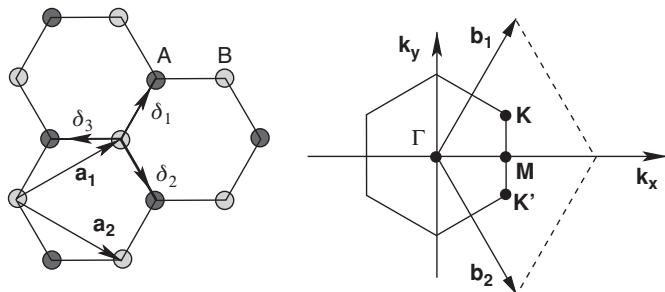
\includegraphics[width=0.7\textwidth]{figs/ch03/fig_3.2.jpg}
\caption*{图 3.2\quad 石墨烯晶格。左图给出原胞基矢$\mathbf a_i$与最近邻格矢量$\boldsymbol\delta_i$；A与B标记石墨烯中两类碳原子。右图给出由格矢量$\mathbf b_i$张成的第一布里渊区。}\label{fig:auto:3.2}
\end{figure}

其中$a=1.42\,\mathrm{\AA}$，为碳–碳最近邻间距。图 3.2 所示的第一布里渊区（first Brillouin zone）由倒格矢量张成

\begin{equation*}
\mathbf b_1 = \frac{2\pi}{3a}\left(1,\sqrt 3\right),\quad \mathbf b_2 = \frac{2\pi}{3a}\left(1,-\sqrt 3\right).
\tag{3.39}
\end{equation*}

第一布里渊区的角点位于

\begin{equation*}
\mathbf K = \frac{2\pi}{3a}\left(1,\frac{1}{\sqrt 3}\right),\quad \mathbf K' = \frac{2\pi}{3a}\left(1,-\frac{1}{\sqrt 3}\right).
\tag{3.40}
\end{equation*}

你需要：(a) 写出该体系的紧束缚哈密顿量并求解其能带；(b) 找出使能量色散为零的$\mathbf k$值（共有两个）；(c) 证明色散可以写成

\begin{equation*}
E(\mathbf q) = \pm\hbar v_{\mathrm F}|\mathbf q|,
\tag{3.41}
\end{equation*}

其中$v_{\mathrm F}=3t/2\hbar a\approx 10^{6}\,\mathrm{m/s}$，$q$是相对于色散过零处动量取值的偏离；(d) 证明在过零点附近，有效哈密顿量可以写成

\begin{equation*}
H \equiv \hbar v_{\mathrm F}\begin{pmatrix} 0 & q_x+\mathrm i q_y \\ q_x-\mathrm i q_y & 0 \end{pmatrix} = \hbar v_{\mathrm F}\,\sigma\cdot\mathbf q
\end{equation*}

的形式，对应$\mathbf K'$点；以及

\begin{equation*}
H \equiv \hbar v_{\mathrm F}\begin{pmatrix} 0 & -q_x+\mathrm i q_y \\ -q_x-\mathrm i q_y & 0 \end{pmatrix} = \hbar v_{\mathrm F}(-q_x\sigma_x + q_y\sigma_y)
\end{equation*}

的形式，对应$\mathbf K$点。

\section*{参考文献}
\addcontentsline{toc}{section}{参考文献}

\begin{itemize}[leftmargin=2em,itemsep=0pt,parsep=0pt,label={}]
\item {[BO1927]} M. Born and J. R. Oppenheimer, Ann. d. Physik 84, 457 (1927).
\item {[W1937]} G. H. Wannier, Phys. Rev. 52, 191 (1937).
\end{itemize}
